\documentclass[pdflatex,compress,mathserif]{beamer}

%\usetheme[dark,framenumber,totalframenumber]{ElektroITK}
\usetheme[darktitle,framenumber,totalframenumber]{ElektroITK}

\usepackage[utf8]{inputenc}
\usepackage[T1]{fontenc}
\usepackage{lmodern}
\usepackage[bahasai]{babel}
\usepackage{amsmath}
\usepackage{amsfonts}
\usepackage{amssymb}
\usepackage{graphicx}
\usepackage{multicol}

\newcommand*{\Scale}[2][4]{\scalebox{#1}{$#2$}}%

\title{PEMODELAN JARINGAN KOMUNIKASI}
\subtitle{Dynamic Routing Protocols}

\author{Tim Dosen Pengampu}

\begin{document}

\maketitle

\section{Dynamic Routing Protocols vs Static Routes}

\begin{frame}
	\frametitle{Dynamic Routing Protocols}
	\begin{itemize}
		\item When a routing protocol is used, routers automatically advertise their
 best paths to known networks to each other.
		\item Routers use this information to determine their own best path to the
 known destinations.
		\item When the state of the network changes, such as a link going down or a
 new subnet being added, the routers update each other.
		\item Routers will automatically calculate a new best path and update the
 routing table if the network changes.
	\end{itemize}
\end{frame}

\begin{frame}{Dynamic Routing Protocols}
	\begin{itemize}
		\item You can get to these networks via me:
	\end{itemize}
	\begin{center}
		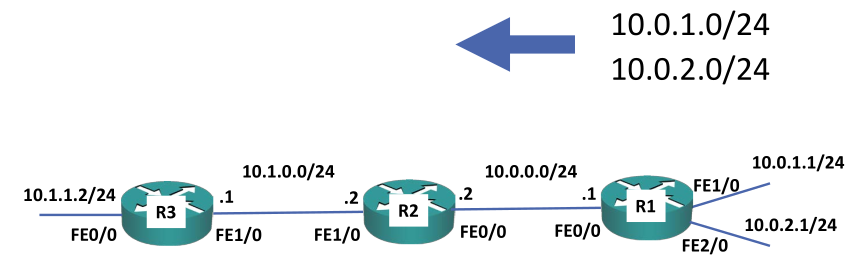
\includegraphics[width=\linewidth]{img/img01}
	\end{center}
\end{frame}

\begin{frame}{Dynamic Routing Protocols}
	\begin{itemize}
		\item Routing Table:
	\end{itemize}
	\begin{center}
		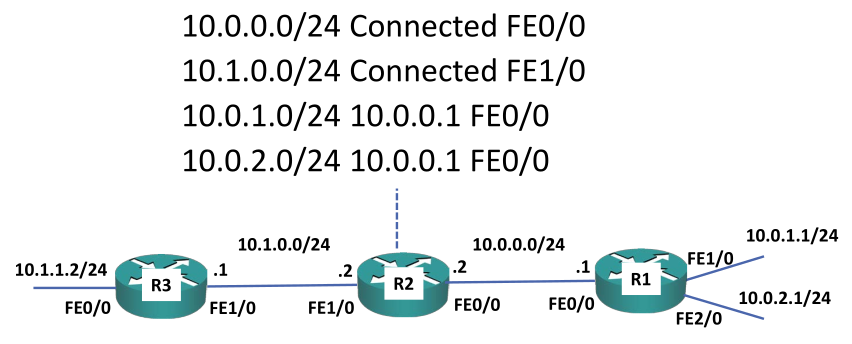
\includegraphics[width=\linewidth]{img/img02}
	\end{center}
\end{frame}

\begin{frame}{Dynamic Routing Protocols}
	\begin{itemize}
		\item You can get to these networks via me:
	\end{itemize}
	\begin{center}
		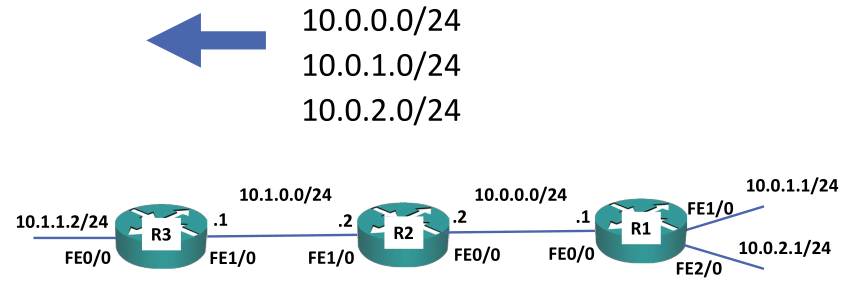
\includegraphics[width=\linewidth]{img/img03}
	\end{center}
\end{frame}

\begin{frame}{Dynamic Routing Protocols}
	\begin{itemize}
		\item Routing Table:
	\end{itemize}
	\begin{center}
		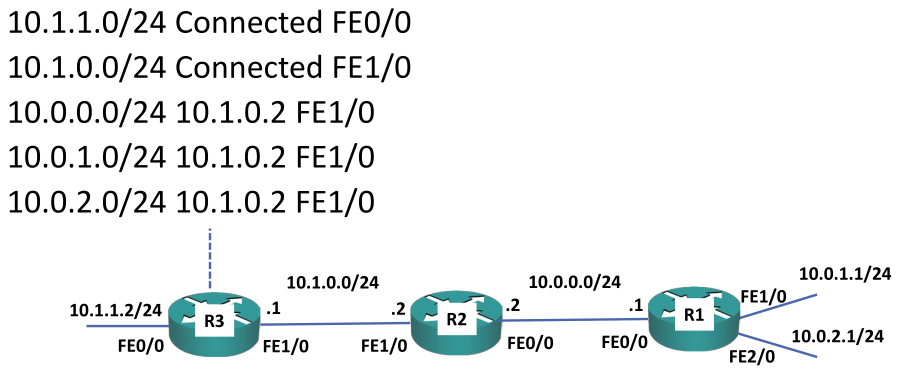
\includegraphics[width=\linewidth]{img/img04}
	\end{center}
\end{frame}

\begin{frame}
	\frametitle{Summary Routes}
	\begin{itemize}
		\item You can get to these networks via me:
	\end{itemize}
	\begin{center}
		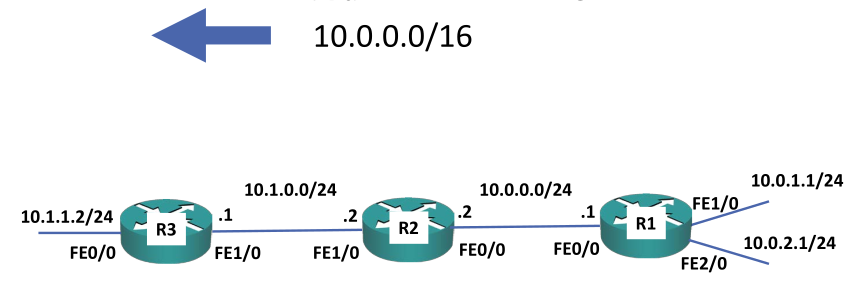
\includegraphics[width=\linewidth]{img/img05}
	\end{center}
\end{frame}

\begin{frame}{Summary Routes}
	\begin{itemize}
		\item Summary routes lead to less memory usage in routers as their routing tables contain less routes
		\item They also lead to less CPU usage as changes in the network only affect
other routers in the same area
		\item For example, if the link on R1 to the 10.0.1.1/24 network goes down, R2
will lose its route there and try to compute a new path
		\item R3 will not be affected as its summary route to 10.0.0.0/16 is unchanged
	\end{itemize}
\end{frame}

\begin{frame}
	\frametitle{Dynamic Routing Protocols\\vs Static Routes}
	\begin{itemize}
		\item Routing protocols are more scalable than administrator defined static
routes.
		\item Using purely static routes is only feasible in very small environments.
	\end{itemize}
\end{frame}

\begin{frame}
	\frametitle{Dynamic Routing Protocol Advantages}
	\begin{itemize}
		\item The routers automatically advertise available subnets to each other
without the administrator having to manually enter every route on every
		router.
		\item If a subnet is added or removed the routers will automatically discover
that and update their routing tables.
		\item If the best path to a subnet goes down routers automatically discover
that and will calculate a new best path if one is available.
	\end{itemize}
\end{frame}

\begin{frame}
	\frametitle{Dynamic Routing Protocols\\vs Static Routes}
	\begin{itemize}
		\item Using a combination of a dynamic routing protocol and static routes is
very common in real world environments.
		\item In this case the routing protocol will be used to carry the bulk of the
network information.
		\item Static routes can also be used on an as needed basis. For example for
backup purposes or for a static route to the Internet (which will typically
be injected into the dynamic routing protocol and advertised to the rest
of the routers.)
	\end{itemize}
\end{frame}

\begin{frame}
	\frametitle{Lab}
	\begin{center}
		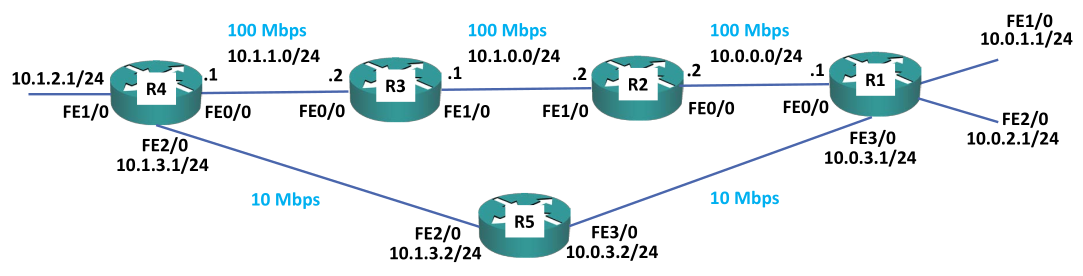
\includegraphics[width=\linewidth]{img/img06}
	\end{center}
\end{frame}

\section{Routing Protocol Types}

\section{Routing Protocol Metrics}

\section{Equal Cost Multi Path}

\section{Administrative Distance}

\section{Loopback Interfaces}

\section{Adjacencies and Passive Interfaces}

\end{document}
